\section{Transactions}\label{transactions}

As there are no miners in the network, transactions are being validated by other nodes that issue transactions themselves. In order to create a new transaction on the network, a node does the following steps:
\begin{enumerate}
    \item The node chooses two unconfirmed transactions (tips) according to a random walk algorithm which will be described in more detail in Section \ref{tip-selection}.
    \item The node is responsible for checking the validity of these two transactions. Conflicting transactions are ignored.
    \item A node has to perform a cryptographic puzzle in order to make the new transaction valid. Similar to the Proof of Work (PoW) mechanism in Bitcoin, this puzzle is solved with computational resources. The puzzle is defined by finding a nonce such that the hash of this number concatenated with some data from the approved transactions results in a number smaller than some predefined constant. This puzzle is necessary in order to prevent several attack scenarios which will be discussed in Chapter \ref{attacks}.
\end{enumerate}

The next section describes parameters which are necessary of the tangle. For all figures, a box resembles a transaction and the directed edge between nodes illustrates the approval of a transactions. In order to understand the approval algorithm, the following five parameters are defined for every transaction.
\begin{description}
    \item[weight] The weight of a transaction is defined by the amount of work that the issuing node has invested in to this transaction. The weight of a transaction resembles its importance. This measurement helps to prevent spamming and other attacks since no node can create an abundance of transactions with meaningful weights within a short period of time. 
    \item[cumulative weight] The cumulative weight of a transaction is calculated by the weight of the transaction itself plus the sum of all transactions that directly or indirectly approve this transaction. Figure \ref{fig:cumulative-weight} shows how the weight and the cumulative weight change after the new transaction \textit{X} is added, the smaller number denotes the weight of a node and the bold number represents cumulative weight of a transaction.\par
        \begin{minipage}{\linewidth}
            \centering
            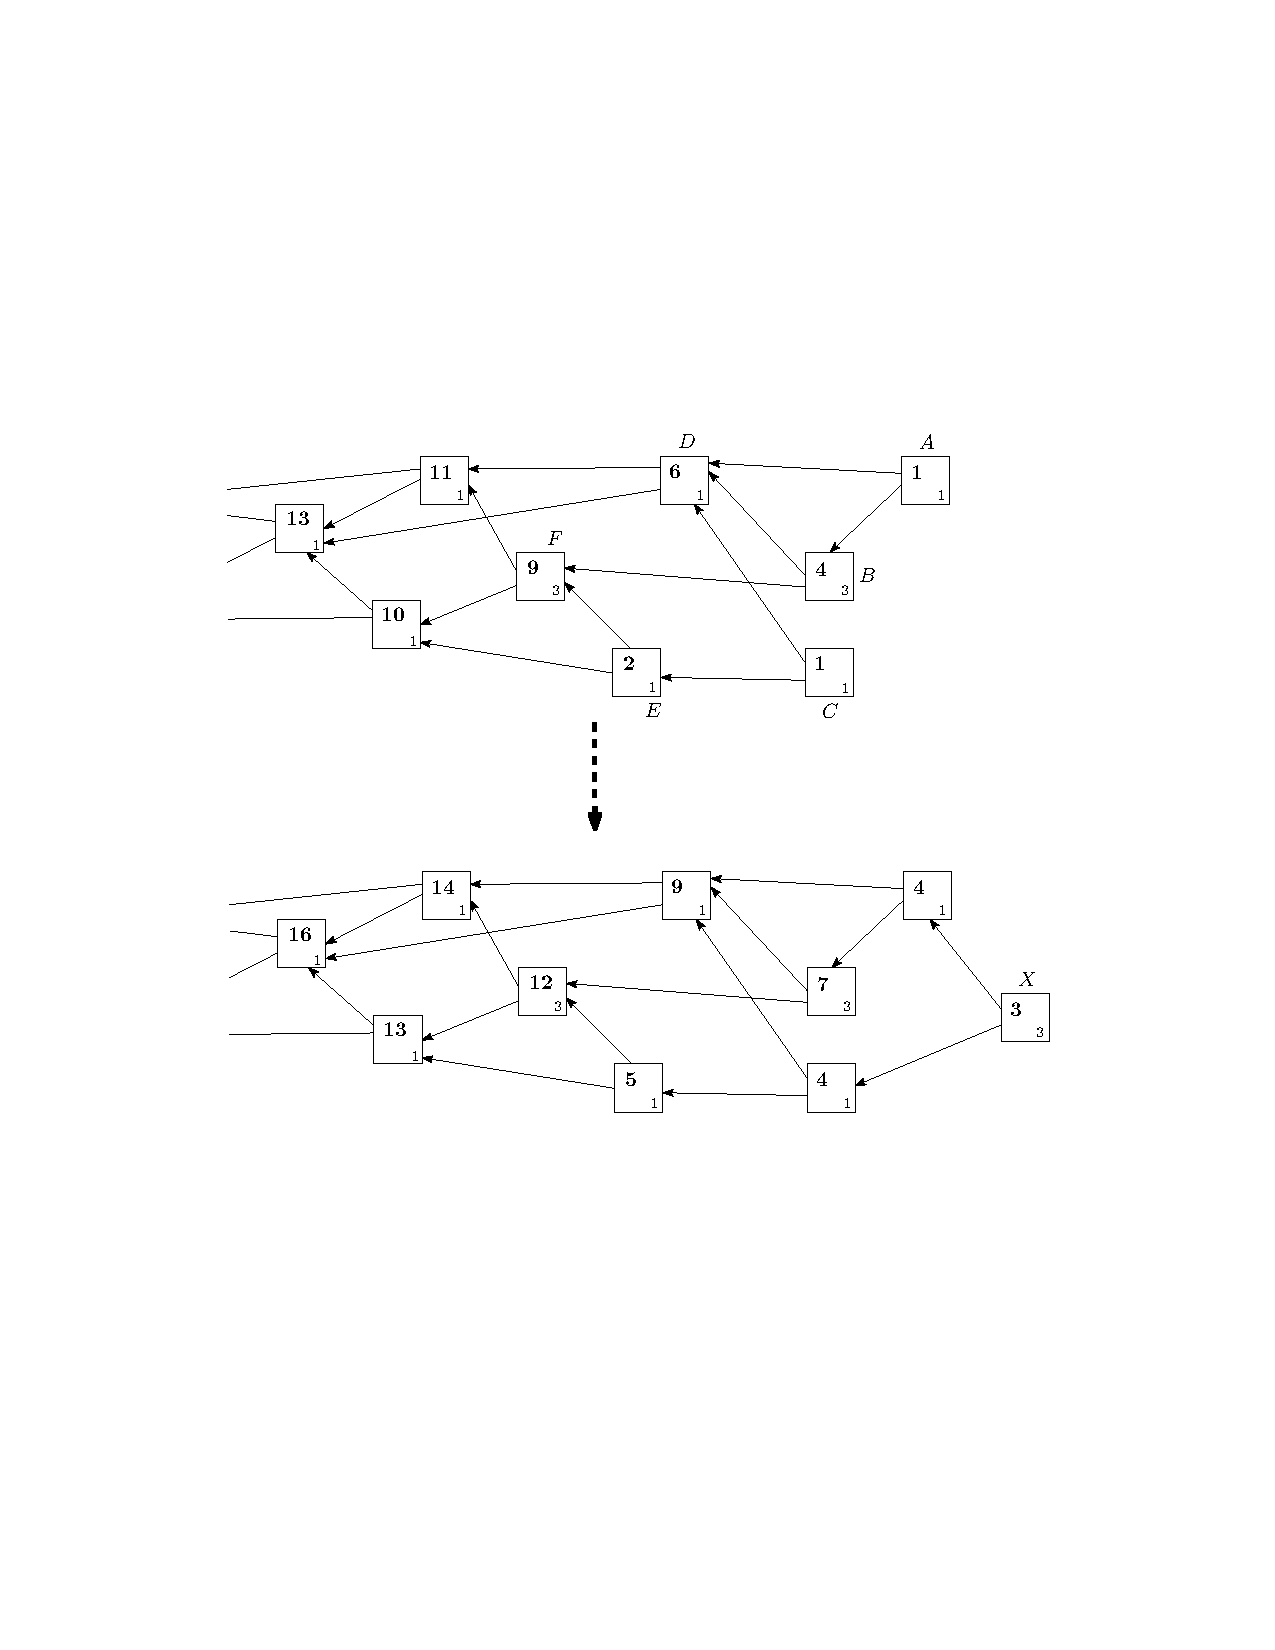
\includegraphics[width=10cm]{images/cummulative_weight.pdf}
            \captionof{figure}{Cumulative Weight \cite{the-tangle}}
            \label{fig:cumulative-weight}
        \end{minipage}
    \item[height] The height of a transaction is the length of the longest oriented path to the genesis transaction. In Figure \ref{fig:height-depth-score}, transaction \textit{G} has a height of 1 due to the blue edge.
    \item[depth] The depth of a transaction is the length of the longest reverse oriented path to some tip. In Figure \ref{fig:height-depth-score}, transaction \textit{G} has a depth of 4 due to the red approvals from newer transactions \textit{F, D, B} and \textit{A}.
    \item[score] The score of a transaction is the sum of weights of all transactions that are approved by this transaction plus its own weight. The scores for transactions \textit{A} and \textit{C} are shown with the circled number in Figure \ref{fig:height-depth-score}.\par
        \begin{minipage}{\linewidth}
            \centering
            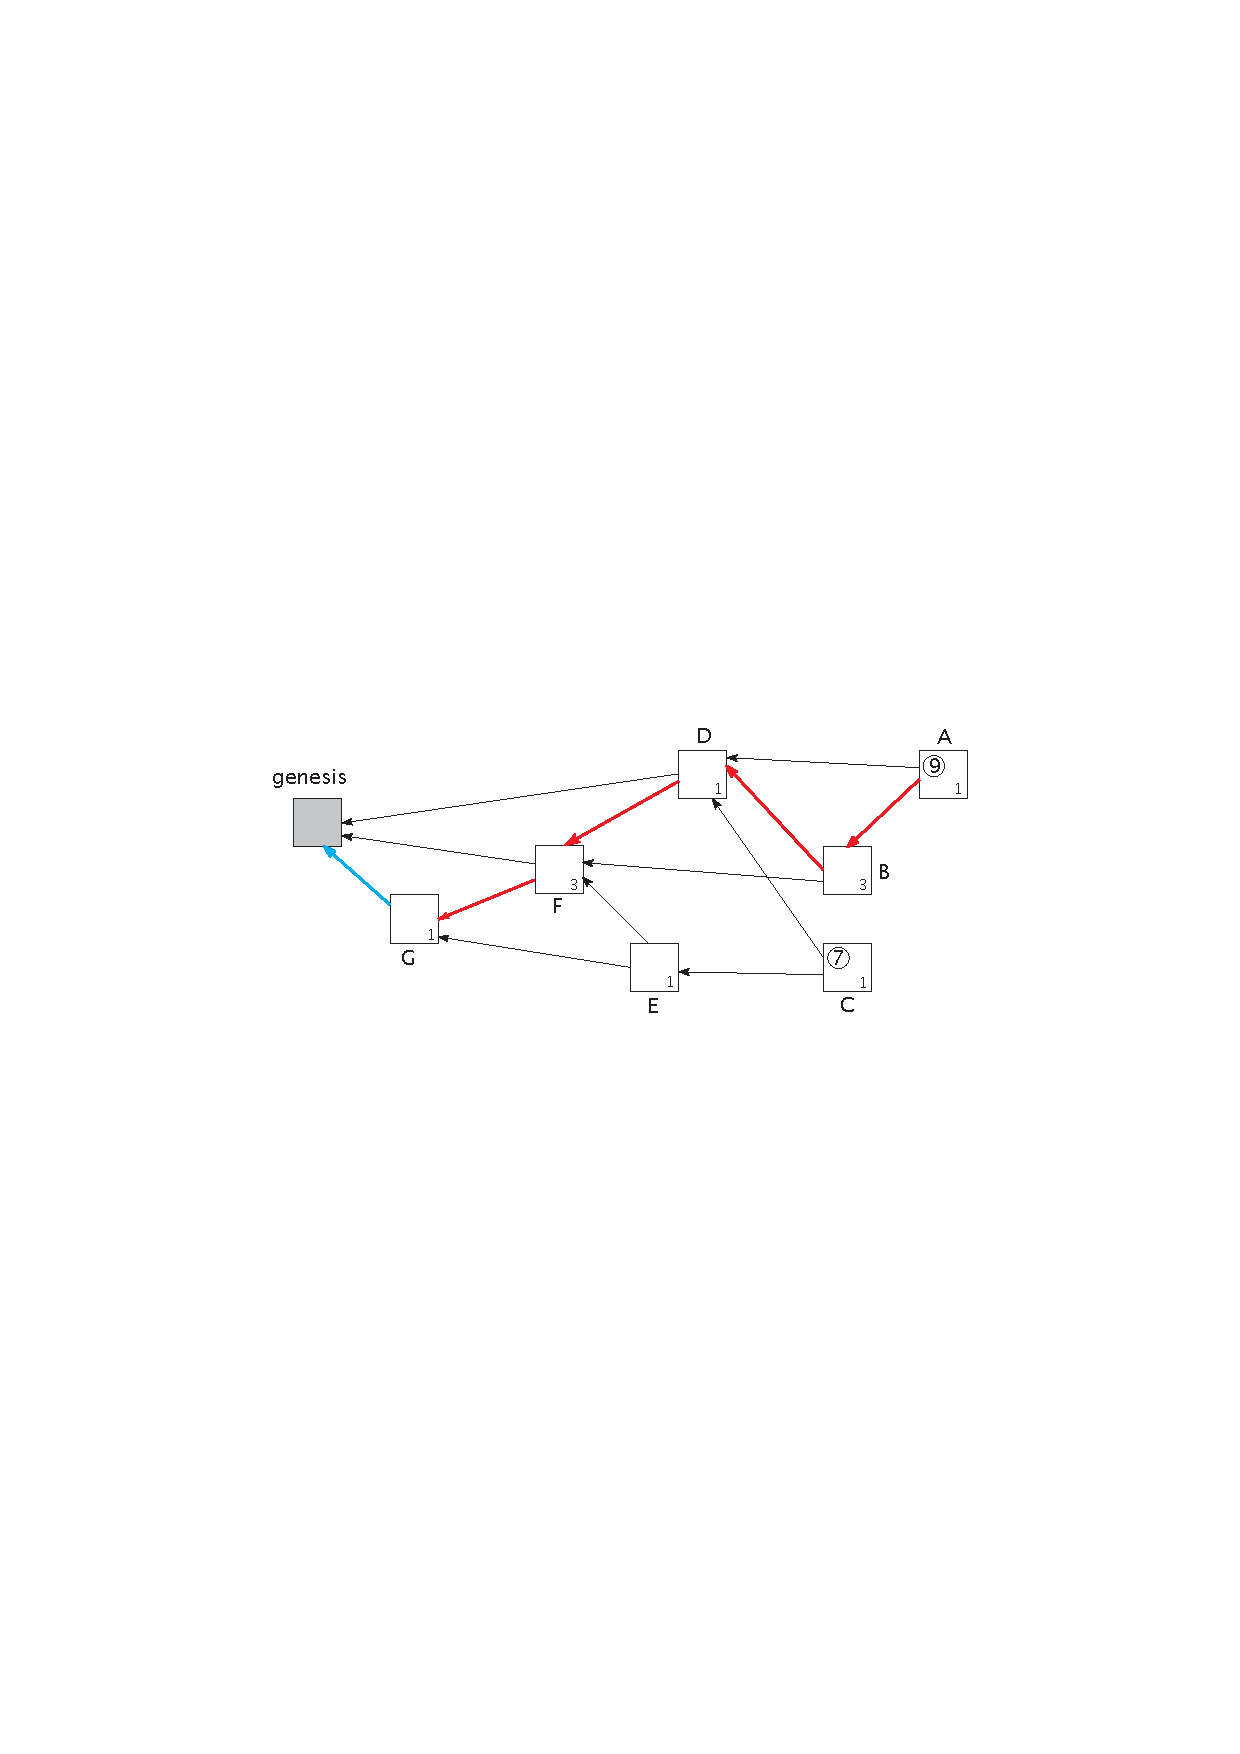
\includegraphics[width=12cm]{images/height-depth-score.pdf}
            \captionof{figure}{Height, Depth and Score \cite{the-tangle}}
            \label{fig:height-depth-score}
        \end{minipage}
\end{description}

These parameters will play an important role when discussing tip selection in Section \ref{tip-selection} and attack scenarios \ref{attacks}.

\subsection{Different Types of Transactions}\label{different-types-of-transactions}

A transaction that facilitates a transfer of IOTAs or stores data on the tangle is a bundle of transactions. Such a bundle is a combination of the following types of transactions:
\begin{description}
    \item[Output transaction] IOTA tokens are sent to another address. The value is always greater than 0 and the address is different than the address issuing the transaction bundle.
    \item[Input transaction with a positive value] These transactions facilitate a transfer to a new address in the sender's wallet.
    \item[Input transaction with a negative value] These transactions completely spend the balance of that account.
    \item[Meta transactions] These transactions have a value of 0 and make use of the \textit{signatureMessageFragment} to store data on the Tangle. 
\end{description}

Each bundle is considered as atomic. Either all or none of the transactions are accepted. Each transaction must provide its own PoW. 


IOTA represents data according to the trinary numeric system. In comparison to binary, a trinary system is more efficient in terms of computation and memory as it can represent data in three states rather than just two. Hence, a transaction is also tryte-encoded where each tryte consists of one of 27 characters.

A transaction in the IOTA protocol consists of 2673 tryte-encoded characters which are equivalent to 1.59 kBytes. Every transaction type contains the same fields. The most interesting fields are the following two.
\begin{description}
    \item[Message (2187 trytes)] This field can be used for two purposes. In case of an input or output transaction, this field contains the signature. In case of a meta transaction, these trytes can be used for storing data on the tangle. If the data is larger than 2187 trytes, the data is split among multiple transactions and grouped together in a transaction bundle. The tangle treats a transaction bundle just like a transaction. It either accepts the bundle or rejects all transactions within the bundle. The tangle explorer cannot search for a specific message. Instead, tags can be used to localize desired messages.
    \item[Tag (27 trytes)] This field is used to search for a transaction with a specific tag value.
\end{description}

Due to the design choice of quantum-resistant signature scheme, the protocol does not allow spending multiple times from the same address. Thus, a simple transaction from Alice's wallet to Bob results in the best case in a transaction bundle of three transactions. One for sending IOTA tokens to Bob, the second one for spending all the remaining IOTAs in Alice's wallet and a third one that is a meta transaction and holds the second part of the signature. Thus, the actual size of a basic Alice-to-Bob transaction results in 8019 trytes (4.77 kBytes).